\documentclass[conference]{IEEEtran}

\usepackage[pdftex]{graphicx}
\graphicspath{{./figures/}}
\DeclareGraphicsExtensions{.pdf,.jpeg,.png}
\usepackage[cmex10]{amsmath}
\usepackage{algorithm,algpseudocode}
\usepackage{hyperref} % must come before url
\usepackage{url}
\usepackage{color} % for \textcolor
\usepackage{subfig} % for \subfloat

\newcommand{\TODO}[1]{
  {\Large \textcolor{red}{\textbf{TODO: }#1}}
}

\begin{document}

% can use linebreaks \\ within to get better formatting as desired
\title{Cost- and Deadline-Constrained Provisioning for Scientific Workflow
Ensembles in IaaS Clouds}


% IEEE Format
\author{\IEEEauthorblockN{Maciej
Malawski\IEEEauthorrefmark{1}\IEEEauthorrefmark{3}, Gideon
Juve\IEEEauthorrefmark{2}, Ewa Deelman\IEEEauthorrefmark{2} and Jarek
Nabrzyski\IEEEauthorrefmark{3}} 
\IEEEauthorblockA{\IEEEauthorrefmark{1}AGH University of Science and
Technology, Dept. of Computer Science, Krakow, Poland, Email:
malawski@agh.edu.pl} 
\IEEEauthorblockA{\IEEEauthorrefmark{2}USC Information Sciences Institute, 4676
Admiralty Way, Marina del Rey, CA, USA, Email: \{gideon,deelman\}@isi.edu} 
\IEEEauthorblockA{\IEEEauthorrefmark{3}University of Notre Dame, Center for
Research Computing, 111 ITC, Notre Dame, IN, USA, Email: naber@nd.edu}
}

% ACM Format
%\numberofauthors{3}
%\author{
%    \alignauthor Maciej Malawski\\
%       \affaddr{AGH University of Science and Technology}\\
%       \affaddr{Dept. of Computer Science}\\
%       \affaddr{Krakow, Poland; and}\\
%       \affaddr{University of Notre Dame}\\
%       \affaddr{Center for Research Computing}\\
%       \affaddr{111 ITC, Notre Dame, IN, USA}\\
%       \email{mmalawsk@nd.edu}
%    \alignauthor Gideon Juve and Ewa Deelman\\
%       \affaddr{USC Information Sciences Institute}\\
%       \affaddr{4676 Admiralty Way}\\
%       \affaddr{Marina del Rey, CA, USA}\\
%       \email{\{gideon,deelman\}@isi.edu}
%    \alignauthor Jarek Nabrzyski\\
%       \affaddr{University of Notre Dame}\\
%       \affaddr{Center for Research Computing}\\
%       \affaddr{111 ITC, Notre Dame, IN, USA}\\
%       \email{naber@nd.edu}
%}

\maketitle
 
\begin{abstract}

Large-scale computational applications represented as scientific workflows, are
often grouped into ensembles composed of several inter-related workflows. In
this paper, we address a new and important problem concerning the efficient 
management of such ensembles under both budget and deadline constraints on 
Infrastructure-as-a-Service (IaaS) clouds. IaaS clouds are characterized by
on-demand resource provisioning capabilities and a pay-per-use model.  We discuss,
develop, and assess algorithms based on static and dynamic strategies for both
task scheduling and resource provisioning. We assume that the workflows within
an ensemble are prioritized by the user. We evaluate the algorithms via
simulation using a set of scientific workflow ensembles with a broad range of
budget and deadline parameters, taking into account uncertainties in task runtime
estimations, provisioning delays and failures. We find that the key 
factor determining the performance of an algorithm is its ability to decide which
workflows in an ensemble to admit or reject for execution. The results
show that the admission procedure based on workflow structure and estimates of
task runtimes can significantly improve the quality of solutions.

\end{abstract}

% IEEE does not have these
%\category{H.3.4}{Systems and Software}{Distributed systems}
%\category{D.4.8}{Performance}{Simulation}
%\terms{DAG, Scheduling, Simulation}
%\keywords{Scientific workflows, Workflow ensembles, Cloud computing, Infrastructure-as-a-Service}

\section{Introduction}
\label{sec:intro}

Scientific workflows, usually represented as directed acyclic graphs (DAGs), are
an important class of applications that lead to challenging problems
in resource management on grid and utility computing systems. Workflows
for large computational problems are often composed of several
inter-related workflows grouped into {\em ensembles}. All the workflows in an
ensemble typically have a similar structure, but they differ in their input
data, number of tasks, and individual task sizes.


The CyberShake~\cite{Callaghan2011} is a good example of an application that
requires scientific workflow ensembles. Generating a hazard map for a region
such as Southern California requires an ensemble of many related workflows to
compute individual hazard curves. E.g. the hazard map generated by the
CyberShake group in 2009 required an ensemble of 239 workflows. In astronomy,
for example, a user might wish to use multiple Montage~\cite{Deelman2008}
workflows with different parameters to generate a set of image mosaics that
cover a given area of the sky in different wavelengths, or use an ensemble to generate
the parts of a very large mosaic. The Pegasus team is now working on a Galactic
Plane project that is focused on generating a mosaic of the entire sky. This
ensemble consists of 17 workflows, each of which contains 900 sub-workflows and
computes one ``tile'' of the full mosaic. Another ensemble example is the
Periodograms application~\cite{Vockler2011} that searches for extrasolar planets
by detecting the periodic dips in light intensity. Due to the large scale of the
input data, this application is often split up into multiple batches processed
by different workflows. Additional workflows are created to run the analysis
using different parameters. A recent analysis of data from the Kepler satellite
required three ensembles of 15 workflows.


Ensemble workflows may differ not only in their parameters, but also in their
priority. For example, in CyberShake some sites may be in heavily populated
areas or in strategic locations such as power plants, while others may be less
important. Scientists typically prioritize the workflows in an ensemble such
that important workflows are finished first. This enables them to see critical
results early, and helps them to choose the most important workflows when the
time and financial resources available for running the computations are limited.

Infrastructure-as-a-Service (IaaS) clouds offer the ability to provision 
computational resources on-demand according to a pay-per-use model. These systems 
are regarded by the scientific community as a potentially attractive source of 
low-cost computing resources~\cite{Ostermann2010, Keahey2009}. In contrast 
to clusters and grids, which typically offer best-effort quality of service, clouds 
give more flexibility in creating a controlled and managed computing environment.
Clouds provide the ability to adjust resource capacity according to the changing
demands of the application, often called auto-scaling. However, giving users 
more control also requires the development of new methods for task 
scheduling and resource provisioning. The resource management decisions required 
in cloud scenarios not only have to take into account traditional performance-related 
metrics such as workflow makespan or resource utilization, but must also now consider
budget constraints, since the resources from public (commercial) clouds
usually have monetary costs associated with them~\cite{Durkee2010}.

In this paper, we aim to gain insight into resource management challenges when
executing scientific workflow ensembles on clouds. In particular, we address a
new and important problem of maximizing the number of completed workflows from
an ensemble under both budget and deadline constraints. The motivation for this
work is to answer the fundamental question of concern to a researcher: How much
computation can be completed given the limited budget and timeframe of a
research project? 

The main contributions of this paper are:
\begin{itemize}
  \item we define the problem of scheduling prioritized workflows grouped
  into ensembles, under both budget and deadline constraints,
  \item we analyze and develop dynamic (on-line) strategies for task scheduling
  and resource provisioning as well as static algorithms that
  rely on the information about the workflow structure (critical paths and
  workflow levels) and estimates of task runtimes. 
  \item we analyze and develop a hybrid workflow-aware dynamic scheduling
  algorithm, together with admission procedures to predict which workflows from
  the ensemble can be completed,
  \item we evaluate these algorithms using our simulator based on
  CloudSim~\cite{Calheiros2011}, which models the infrastructure and the application, 
  taking into account uncertainties in task runtime
  estimations, provisioning delays and failures, 
  \item we discuss the performance of the algorithms on a set of
  synthetic workflow ensembles based on important, real scientific
  applications, on a broad range of different application scenarios and
  varying constraint values.
\end{itemize}



The paper is organized as follows: after an analysis of related work in
Section~\ref{sec:related}, Section~\ref{sec:problem} describes the
infrastructure and application model we are targeting in this paper. In
Section~\ref{sec:algorithms} we describe the dynamic and static algorithms we
developed. Section~\ref{sec:performance} presents test scenarios and performance
metrics, while Section~\ref{sec:results} discusses the results of simulation
studies of these algorithms. Finally, general conclusions, lessons learned, and
future work are outlined in Section~\ref{sec:conclusions}.


\section{Related Work}
\label{sec:related}
General policy and rule-based approaches to dynamic provisioning (e.g. Amazon
Auto Scaling~\cite{Autoscaling} and
RightScale~\cite{RightScale}) allow adjusting the size
of resource pool based on metrics related to infrastructure and application.
A typical infrastruc\-ture-specific metric is system load, whereas
application-speci\-fic metrics include response time and length of a task or
of a request queue. It is possible to set thresholds and limits to tune the behavior
of these autoscaling systems, but no support for complex applications is provided.

Policy-based approaches for scientific workloads (e.g. \cite{Marshall2010,
Kim2011}) also allow to scale the cloud resource pool or to extend the
capabilities of clusters using cloud-burst techniques. Our approach is different
in that we consider workflows, while policy based approaches typically consider
bags of independent tasks or unpredictable batch workloads. Our approach enables us to
take advantage of workflow-aware scheduling heuristics that cannot be applied to
independent tasks.


Our work is related to the strategies for deadline-con\-strained
cost-minimization workflow scheduling, developed for utility grid systems. However, our problem is
different from \cite{Yu2005, Abrishami2010} in that we consider ensembles of workflows in
IaaS clouds, which allow one to provision resources on a per-hour billing model,
rather than utility grids, which allow one to choose from a pool of existing
resources with a per-job billing model. Our work is also different from
cloud-targeted autoscaling solution~\cite{Mao2011} in that we consider ensembles
of workflows rather than unpredictable workloads containing workflows. We also consider budget constraints
rather than cost minimization as a goal. In other words, we assume that there is
more work to be done than the available budget, so some work must be rejected.
Therefore cost is not something we optimize (i.e. an objective), but rather a constraint.


This work is related to bi-criteria scheduling and multi-criteria scheduling of
workflows~\cite{Wieczorek2009,Prodan2010,Dongarra2007}. These approaches are
similar to ours in that we have two scheduling criteria: cost and makespan. The
challenge in multi-criteria scheduling is to derive an objective function that
takes into account all of the criteria. In our case one objective (amount
of work completed) is subject to optimization, whereas time and cost are
treated as constraints. Other approaches~\cite{Talukder2009,Pandey2010} use
metaheuristics that usually run for a long time before producing good results,
which makes them less useful in the scenarios we consider in this paper. Our work can be also
regarded as an extension of the budget-constrained workflow scheduling
\cite{Sakellariou2007} in the sense that we are dealing with workflow ensembles
and the deadline constraint is added.

 
\section{Problem Description}
\label{sec:problem}

\subsection{Resource Model}

We assume a resource model similar to Amazon's Elastic Compute Cloud (EC2),
where virtual machine (VM) instances are requested on-demand and are billed by
the hour, with partial hours being rounded up. Although there may be
heterogeneous VM types with different amounts of CPU, memory, disk space, and
I/O, for this paper we focus on a single VM type because we assume that for most
applications there will typically be only one or two VM types with the best
price/performance ratio for the application~\cite{Juve2009}. We also assume that
a submitted task has exclusive access to a VM instance and that there is no
preemption. We assume that there is a delay between the time that a new VM
instance is requested and when it becomes available to execute tasks. In
practice this delay is typically on the order of tens of seconds to a few
minutes, and is highly dependent upon the cloud platform and the VM image
size~\cite{Nurmi2008b}.



\subsection{Application Model}

The target applications are ensembles of scientific workflows that can be
modeled as Directed Acyclic Graphs (DAGs), where the nodes in the graph
represent computational tasks, and the edges represent data- or control-flow
dependencies between the tasks. We assume that there are runtime estimates for
each task in the workflow based on either a performance model of the
application, or historical data that can be mined. Additionally, we assume that
the runtime estimates for individual workflow tasks are not perfect, but may
vary based on a uniform distribution of $\pm p\%$.


This study uses synthetic workflows that were generated using historical data
from real applications~\cite{Bharathi2008}. The applications come from a wide
variety of domains including: bioinformatics (Epigenomics, SIPHT: sRNA
identification protocol using high-throughput technology), astronomy (Montage),
earthquake science (CyberShake), and physics (LIGO). The runtimes used to
generate the synthetic workflows are based on distributions gathered from
running real workflows. The synthetic workflows were generated using code
developed by Bharathi, et al~\cite{WorkflowGenerator}.


Although scientific workflows are often data-intensive, the algorithms described
in the next section do not currently consider the size of input and output data
when scheduling tasks. Instead it is assumed that all workflow data is stored in
a shared cloud storage system, such as Amazon S3, and that intermediate data
transfer times are included in task runtime estimates. It is also assumed that
data transfer times between the shared storage and the VMs are equal for
different VMs so that task placement decisions do not have an impact on the
runtime of the tasks.


A workflow ensemble consists of several related workflows that a user wishes to
run. Each workflow in an ensemble is given a numeric priority that indicates how
important the workflow is to the user. As such, the priorities indicate the
utility function of the user. These priorities are absolute in the sense that
completing a workflow with a given priority is more valuable (gives the user
more utility) than completing all other workflows in the ensemble with lower
priorities combined. The goal of the workflow ensemble scheduling and cloud
provisioning problem is to complete as many high-priority workflows as possible
given a fixed budget and deadline. Only workflows for which all tasks are
finished by the deadline are considered to be complete---partial results are not
usable in this model.



\section{Algorithms}
\label{sec:algorithms}

This section describes three algorithms were developed to schedule and provision resources for ensembles of workflows on the cloud under budget and deadline constraints.

\subsection{Dynamic Provisioning Dynamic Scheduling (DPDS)}
\label{sec:dpds}

DPDS is an online algorithm that provisions resources and schedules tasks at
runtime. It consists of two main parts: a provisioning procedure, and a
scheduling procedure.


DPDS' provisioning procedure is based on resource utilization. DPDS starts with
a fixed number of resources calculated based on the available time and budget,
and adjusts the number of resources according to how well they are utilized by
the application.
Given a budget in dollars $b$, deadline in hours $d$, and the hourly price of a
VM in dollars $p$, it is easy to calculate the number of VMs, $N_{VM}$, to
provision so that the entire budget is consumed before the deadline:
\begin{equation}
\label{eq:static-plan}
N_{VM} = \lceil b / (d * p) \rceil
\end{equation}
%
The DPDS algorithm provisions $N_{VM}$ VMs at the start of the ensemble execution.


The DPDS algorithm periodically computes resource
utilization using the percentage of idle VMs over time, and adjusts the number
of VMs if the utilization is above or below given thresholds. Because it is
assumed that VMs are billed by the hour, DPDS only considers VMs that are
approaching their hourly billing cycle when deciding which VMs to terminate.
This dynamic provisioning algorithm is shown in Algorithm~\ref{alg:prov}.


\begin{algorithm}[tb]
\caption{Dynamic provisioning algorithm for DPDS}
\label{alg:prov}
{\footnotesize
\begin{algorithmic}[1]
\Require $c$: consumed budget; $b$: total budget; $d$: deadline; $p$: price;
$t$: current time; $u_h$: upper utilization threshold; $u_l$: lower utilization
threshold; $v_{max}$: maximum number of VMs
\Procedure{Provision}{}
  \State $V_R\gets$ set of running VMs
    \State $V_C\gets$ set of VMs completing billing cycle
    \State $V_T\gets \emptyset$ \Comment{set of VMs to terminate}
    \State $n_T\gets 0$ \Comment{number of VMs to terminate}
    \If{$ b - c < |V_C| * p\ or\ t > d $ }
      \State $n_T\gets |V_R| - \lfloor(b-c)/p\rfloor$
      \State $V_T\gets$ select $n_T$ VMs to terminate from $V_C$
      \State \Call{Terminate}{$V_T$} \label{l:terminate1}
    \Else 
    \State $u\gets$ current VM utilization
      \If{$u>u_h$ and $|V_R| < v_{max}*N_{VM}$}
        \State \Call{Start}{$new\ VM$}
      \ElsIf{$u<u_l$}
        \State $V_I\gets$ set of idle VMs
        \State $n_T\gets \lceil|V_I|/2\rceil$ \label{l:nT2}
      \State $V_T\gets$ select $n_T$ VMs to terminate from $V_I$
        \State \Call{Terminate}{$V_T$} \label{l:terminate2}
      \EndIf 
    \EndIf
\EndProcedure
\end{algorithmic}
}
\end{algorithm}

The set of VMs completing their billing cycle is determined by  both
the provisioner interval, and the termination delay of the provider. This
guarantees that VMs can be terminated before they start the next billing cycle
and prevents the budget from being overrun. The VMs terminated in line
\ref{l:terminate1} of Algorithm~\ref{alg:prov} are the ones that would overrun
the budget if not terminated in the current provisioning cycle. The VMs
terminated in line \ref{l:terminate2} are chosen to increase the resource
utilization to the desired threshold. In order to prevent instances that have
already been paid for from being terminated too quickly, no more than half of
the idle resources are terminated during each provisioning cycle. To avoid an
uncontrolled increase in the number of instances, which may happen in the case
of highly parallel workflows, the provisioner will not start a new VM if the
number of running VMs is greater than the product of $N_{VM}$ (from
Equation~\ref{eq:static-plan}) and an autoscaling parameter, $v_{max}$. Unless
otherwise specified, $v_{max}$ is assumed to be 1.


In order to schedule individual workflow tasks onto available VMs, DPDS uses the
dynamic, priority-based scheduling procedure shown in Algorithm~\ref{alg:ds}.
Initially, the ready tasks from all workflows in the ensemble are added to a
priority queue based on the priority of the workflow to which they belong. If
there are idle VMs available, and the priority queue is not empty, the next task
from the priority queue is submitted to an arbitrarily chosen idle VM. The
process is repeated until there are no idle VMs or the priority queue is empty.
The scheduler then waits for a task to finish, adds its ready children to the
priority queue, marks the VM as idle, and the entire process repeats until the
deadline is reached.

\begin{algorithm}[tb]
\caption{Priority-based scheduling algorithm for DPDS}
\label{alg:ds}
{\footnotesize
\begin{algorithmic}[1]
\Procedure{Schedule}{}
    \State $P\gets$ empty priority queue
	\State $IdleVMs\gets$ set of idle VMs
	\For{root task $t$ in all workflows}
    	\State \Call{Insert}{$t,P$} 
    \EndFor
    \While{deadline not reached}
    	\While{$IdleVMs \neq \emptyset\ and\ P \neq \emptyset$}
    		\State $v\gets$ \Call{SelectRandom}{$IdleVMs$}
    		\State $t\gets$ \Call{Pop}{$P$}
    		\State \Call{Submit}{$t,v$}
    	\EndWhile
    	\State Wait for task $t$ to finish on VM $v$
    	\State Update $P$ with ready children of $t$
		\State \Call{Insert}{$v,IdleVMs$}
    \EndWhile
\EndProcedure
\end{algorithmic}
}
\end{algorithm}


The DPDS algorithm guarantees that tasks from lower priority workflows are
always deferred when higher-priority tasks are available, but lower-priority
tasks can still occupy idle VMs when higher-priority tasks are not available.
However, because there is no preemption, long-running low-priority tasks may
delay the execution of higher-priority tasks. In addition, tasks from low
priority workflows may be executed even though there is no chance that those
workflows will be completed within the current budget and deadline.
Figure~\ref{fig:algorithm-example}a shows an example schedule generated using
the DPDS algorithm. The figure illustrates how tasks from lower priority workflows
backfill idle VMs when tasks from higher priority workflows are not available.



\subsection{Workflow-Aware DPDS (WA-DPDS)}

The DPDS algorithm does not use any information about the structure of the
workflows in the ensemble when scheduling tasks: it looks only at the priorities
of the ready tasks when deciding which task to schedule next. It does not
consider whether a lower priority task belongs to a workflow that will never be
able to complete given the current budget and deadline. As a result, DPDS may
start lower priority tasks just to keep VMs busy that will end up delaying
higher priority tasks later on, making it less likely that higher priority
workflows will be able to finish.


In order to address this issue, the Workflow-Aware DPDS (WA-DPDS) algorithm
extends DPDS by introducing a workflow admission procedure. The admission
procedure is invoked whenever WA-DPDS sees the first task of a new workflow at
the head of the priority queue (i.e. when no other tasks from the workflow have
been scheduled yet). The admission procedure---shown in
Algorithm~\ref{alg:wa-dpds}---estimates whether there is enough budget remaining
to admit the new workflow; if there is not, then the workflow is rejected and
its tasks are removed from the queue. This algorithm compares the current cost
(consumed budget) and remaining budget, taking into account the cost of
currently running VMs, and the cost of workflows that have already been
admitted. In addition, it adds a small safety margin of \$0.10 to avoid going
over the budget.


\begin{algorithm}[tb]
\caption{Workflow admission algorithm for WA-DPDS}
\label{alg:wa-dpds}
{\footnotesize
\begin{algorithmic}[1]
\Require $w$: workflow; $b$: budget; $c$: current cost
\Procedure{Admit}{$w,b,c$}
    \State $r_n\gets b-c$ \Comment{Budget remaining for new VMs}
    \State $r_c\gets $cost committed to VMs that are running
    \State $r_a\gets $cost to complete workflows previously admitted
  \State $r_m\gets 0.1$ \Comment{Safety margin}
  \State $r_b\gets r_n+r_c-r_a-r_m$ \Comment{Budget remaining}
  \State $c_w\gets$ \Call{EstimateCost}{w}
    \If{$c_w<r_b$}  \textbf{return} $TRUE$
    \Else ~  \textbf{return} $FALSE$
  \EndIf       
\EndProcedure
\end{algorithmic}
}
\end{algorithm}

This admission procedure relies only on the total estimated resource consumption
and compares it to the remaining budget. We found that this estimation is useful
not only to prevent low-priority workflows from delaying high-priority ones, but
also to reject large and costly workflows that would overrun the budget and
admit smaller workflows that can efficiently utilize idle resources.
% in
%ensembles containing workflows of non-uniform sizes. It would also be possible
%to extend this admission procedure to check other constraints, such as whether
%the estimated critical path of the new workflow exceeds the time remaining
%until the deadline.



\subsection{Static Provisioning Static Scheduling (SPSS)}

The previous dynamic (online) algorithms make provisioning and scheduling
decisions at runtime. In comparison, the SPSS algorithm creates a provisioning
and scheduling plan before running any workflow tasks. This enables SPSS to
start only those workflows that it knows can be completed given the deadline and
budget constraints, and eliminates any waste that may be allowed by the dynamic
algorithms. However, the disadvantage of SPSS is that it is sensitive to dynamic
changes in the environment (see Sections~\ref{sec:delays} and
\ref{sec:variances}).


The approach used by SPSS is to plan each workflow in the ensemble in priority
order, rejecting any workflows that would exceed the dedline or budget. Once the
plan is complete, the VMs are provisioned and tasks are executed according to
the schedules given by the plan.


%The disadvantage of the static planning approach used by SPSS is that it is
%sensitive to dynamic changes in the environment and the application that may
%disrupt its carefully constructed plan. For example, if there are provisioning
%delays, or if the runtime estimates for the tasks are inaccurate, then workflow
%execution may diverge from the plan. This issue will be discussed further in
%Sections~\ref{sec:delays} and \ref{sec:variances}.


Algorithm~\ref{alg:admit} shows how ensembles are planned in SPSS. Workflows
from the ensemble are considered in priority order. For each workflow, SPSS
attempts to build on top of the current plan by provisioning VMs to schedule the
tasks of the workflow so that it finishes before the deadline with the least
possible cost. If the cost of the new plan is less than the budget, then the new
plan is accepted and the workflow is admitted. If not, then the new plan is
rejected and the process continues with the next workflow in the ensemble. The
idea is that, if each workflow can be completed by the
deadline with the lowest possible cost, then the number of workflows that can be
completed within the given budget will be maximized.


To plan a workflow, the SPSS algorithm assigns sub-deadlines to each individual
task in the workflow, and then schedules each task so as to minimize the cost of
the task while still meeting its assigned sub-deadline. If each task can be
completed by its deadline in the least expensive way, then the cost of the
entire workflow can be minimized without exceeding the deadline. SPSS assigns
sub-deadlines to each task based on the slack time of the workflow, which is
defined as the amount of extra time that a workflow can extend its critical path
and still be completed by the ensemble deadline. For a workflow $w$, the slack
time of $w$ is:
$$ ST(w) = d - CP(w) $$
where $d$ is the deadline and $CP(w)$ is the critical path of $w$. We
assume that $CP(w) \leq d$, otherwise the workflow cannot be completed by the
deadline and must be rejected. 
%For large ensembles we expect the critical path
%of any individual workflow to be much less than the deadline.


\begin{algorithm}[tb]
\caption{Ensemble planning algorithm for SPSS}
\label{alg:admit}
{\footnotesize
\begin{algorithmic}[1]
\Require $W$: workflow ensemble; $b$: budget; $d$: deadline
\Ensure Schedule as much of $W$ as possible given $b$ and $d$
\Procedure{PlanEnsemble}{$W,b,d$}
    \State $P\gets \emptyset$ \Comment{Current plan}
    \State $A\gets \emptyset$ \Comment{Set of admitted DAGs}
    \For{$w\ in\ W$}
        \State $P^\prime \gets$\ \Call{PlanWorkflow}{$w,P,d$}
        \If{$Cost(P^\prime) \le b$}
            \State $P\gets\ P^\prime$ \Comment{Accept new plan}
            \State $A \gets A\ +\ w$ \Comment{Admit w}
        \EndIf
    \EndFor
    \State \textbf{return} $P,A$
\EndProcedure
\end{algorithmic}
}
\end{algorithm}

A task's level is the length of the longest path between the task and an entry task of the workflow:
%
$$
Level(t) = \begin{cases}
0,&$if~$Pred(t) = \emptyset\cr
\max_{p \in Pred(t)}Level(p)+1,&$otherwise.$
\end{cases}
$$
%
SPSS distributes the slack time of the workflow by level, so that each level of the workflow gets a portion of the workflow's slack time proportional to the number of tasks in the level and the total runtime of tasks in the level. The idea is that levels containing many tasks and large runtimes should be given a larger portion of the slack time so that tasks in those levels may be serialized. Otherwise, many resources need to be allocated to run all of the tasks in parallel, which may be more costly.

The slack time of a level $l$ in workflow $w$ is given by:
%
$$
ST(l) = ST(w) \Biggl[\left({\alpha}\frac{N(l)}{N(w)}\right) + \left({(1 - \alpha)}\frac{R(l)}{R(w)} \right)\Biggr]
$$
%
where $N(w)$ is the number of tasks in the workflow, $N(l)$ is the number of tasks in level $l$, $R(w)$ is the total runtime of all tasks in the workflow, $R(w)$ is the total runtime of all tasks in level $l$, and $\alpha$ is a parameter between 0 and 1 that causes more slack time to be given to levels with more tasks (large $\alpha$) or more runtime (small $\alpha$).

The deadline of a task $t$ is then:
%
$$
DL(t) = LST(t) + RT(t) + ST(Level(t))
$$
%
where $Level(t)$ is the level of $t$, $RT(t)$ is the runtime of $t$, and $LST(t)$ is the latest start time of $t$ determined by:
%
$$
LST(t) = \begin{cases}
0,&$if~$Pred(t) = \emptyset\cr
\max_{p \in Pred(t)} DL(p),&$otherwise.$
\end{cases}
$$

\begin{algorithm}[tb]
\caption{Workflow planning algorithm for SPSS}
\label{alg:planworkflow}
{\footnotesize
\begin{algorithmic}[1]
\Require $w$: workflow; $P$: current plan; $d$: deadline
\Ensure Create plan for $w$ that minimizes cost and meets deadline $d$
\Procedure{PlanWorkflow}{$w,P,d$}
    \State $P^\prime\gets$ copy of $P$
    \State \Call{DeadlineDistribution}{w,d}
    \For{$t\ in\ w\ sorted\ by\ DL(t)$}
        \State $v \gets$ VM that minimizes cost and start time of t
        \If{$FinishTime(t,v) < DL(t)$}
            \State Schedule(t,v)
        \Else
            \State Provision a new VM v
            \State Schedule(t,v)
        \EndIf
    \EndFor
    \State \textbf{return} $P^\prime$
\EndProcedure
\end{algorithmic}
}
\end{algorithm}


Algorithm~\ref{alg:planworkflow} shows how SPSS creates low-cost plans for each
workflow. The \textsc{PlanWorkflow} procedure first calls
\textsc{DeadlineDistribution} to assign sub-deadlines to tasks.
% according to the procedure described above. 
Then, \textsc{PlanWorkflow} schedules
tasks onto VMs, allocating new VMs when necessary. For each task in the
workflow, the least expensive slot is chosen to schedule the task so that it can
be completed by  its deadline. VMs are allocated in blocks of one billing cycle
(one hour) regardless of the size of the task. When computing the cost of
scheduling a task on a given VM, the algorithm considers idle slots in blocks
that were allocated for previous tasks to be free, while slots in new blocks
cost the full price of a billing cycle. 
%For example, if a task has a runtime of
%10 minutes, and the price of a block is \$1, then the algorithm will either
%schedule the task on an existing VM that has an idle slot larger than 10
%minutes for a cost of \$0, or it will allocate a new block on an existing VM,
%or provision a new VM, for a cost of \$1. 
If the cost of slots on two different
VMs is equal, then the slot with the earliest start time is chosen. To prevent too
many VMs from being provisioned, the algorithm always prefers to extend the
runtime of existing VMs before allocating new VMs. 
%The result of this is that
%the algorithm will only allocate a new block if there are no idle slots on
%existing blocks large enough or early enough to complete the task by its
%deadline, and it will only allocate a new VM if it cannot add a block to an
%existing VM to complete the task by its deadline.

\begin{figure}[tb] 
  \centering
  \subfloat[DPDS]{
  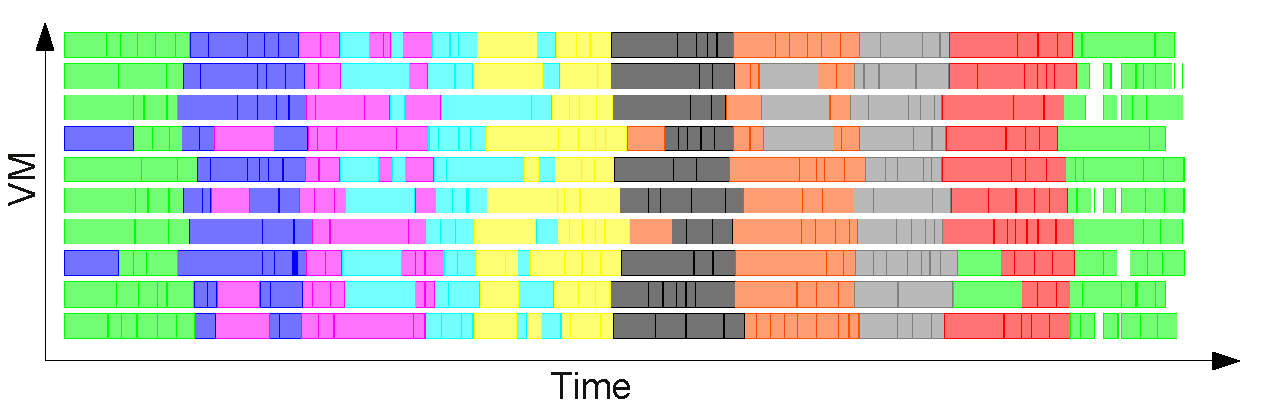
\includegraphics[width=0.45\textwidth]{figures/spds-gantt}
  }\\
  \subfloat[SPSS]{
  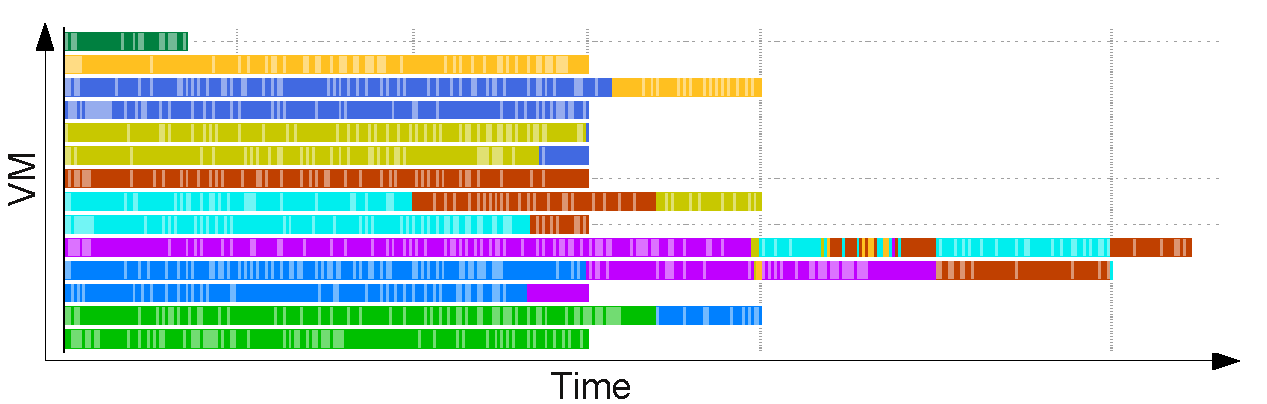
\includegraphics[width=0.45\textwidth]{figures/spss-gantt}
  }
  \caption[Example schedules generated by the algorithms]{Example
  schedules generated by the algorithms. Each row is a different
  VM. Tasks are represented as boxes and are colored by workflow.}
  \label{fig:algorithm-example}
\end{figure}


An example schedule generated by SPSS (Figure~\ref{fig:algorithm-example}b)
shows how SPSS tends to start many workflows in parallel, running each workflow
over a longer period of time on only a few VMs to minimize cost. In comparison,
the dynamic algorithms tend to run one workflow at a time across many VMs in
parallel.


\section{Evaluation Methods}
\label{sec:performance}


\subsection{Simulator}

To evaluate and compare the three proposed algorithms, we developed a cloud
workflow simulator based on CloudSim~\cite{Calheiros2011}. Our simulation model
consists of Cloud, VM and WorkflowEngine entities. The Cloud entity starts and
terminates VM entities using an Amazon EC2-like API. VM entities simulate the
execution of individual tasks, including randomized variations in runtime. The
WorkflowEngine entity manages the scheduling of tasks and the provisioning of 
VMs based on the chosen algorithm. We assume that the VMs have a single core
and execute tasks sequentially. 
%Although CloudSim provides a more advanced infrastructure model which includes
%time-sharing and space-sharing policies, we do not use these features since we
%are interested mainly in the execution of tasks on VMs and high-level workflow
%scheduling and provisioning. 
The simulator reads workflow description files in
a modified version of the DAX format used by the Pegasus Workflow Management
System~\cite{Deelman2005}. 
%The modified file format was created for the
%synthetic workflow generator developed by Bharathi, et al~\cite{Bharathi2008}.


\subsection{Workflow Ensembles}
\label{sec:ensembles}


In order to evaluate the algorithms on a standard set of workflows, we created
randomized ensembles using workflows available from the workflow generator
gallery published online by Bharathi, et al~\cite{WorkflowGenerator}. The
gallery contains synthetic workflows modeled using structures and parameters
that were taken from real applications. Ensembles were created using synthetic
workflows from five real applications: SIPHT, LIGO, Epigenomics, Montage and
CyberShake. For each of these applications, workflows with 50, 100, 200, 300,
400, 500, 600, 700, 800, 900 and 1000 tasks were generated. For each workflow
size, 20 different workflow instances were generated using parameters and task
runtime distributions from traces of real workflows. The total collection of
synthetic workflows contains 5 applications, 11 different workflow sizes, and 20
workflow instances, for a total of 1100 synthetic workflows.


Using this collection of workflows, we constructed five different ensemble types:
%
%\begin{itemize}
constant, uniform sorted, uniform unsorted, Pareto sorted and Pareto unsorted.
%\end{itemize}
In the unsorted ensembles, workflows of different sizes are mixed together, and
the priorities are assigned randomly.
% so that there is no relationship between
%priority and workflow size. 
For many applications, however, large workflows are
more important to users than small workflows because they represent more
significant computations. To model this, the sorted ensembles are sorted by
size, so that the largest workflows have the highest priority.


Constant ensembles contain workflows that all have the same number of tasks. 
%For each constant ensemble, 
The number of tasks is chosen randomly from the set of
possible workflow sizes. Once the size is determined, then N workflows of that
size are chosen randomly for the ensemble from the set of synthetic workflows.
%for the given application.


Uniform ensembles contain workflows with sizes that are uniformly distributed
among the set of possible sizes. Each workflow 
%in a uniform ensemble 
is selected by first randomly choosing the size the workflow
% according to a uniform distribution, 
and then randomly choosing a workflow of that size from the set of
synthetic workflows.
% for the given application.


Pareto ensembles contain a small number of larger workflows and a large number
of smaller workflows. Their sizes  
%in a Pareto ensemble 
are chosen according to a Pareto distribution. The distribution was modified so
that the number of large workflows (of size $\geq$ 900) is increased by a small amount to
produce a ``heavy-tail''. This causes Pareto ensembles to have a slightly larger
number of large workflows, which reflects behavior commonly observed in many
computational workloads. 
%An example of the distribution of workflow sizes that
%occurs in a Pareto ensemble is shown in Figure~\ref{fig:ensemble-pareto}.


%\begin{figure}[ht] 
%    \centering
%    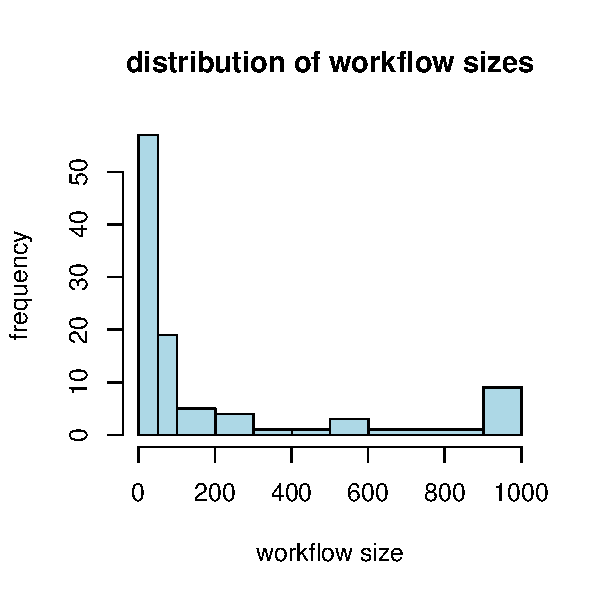
\includegraphics[width=0.6\columnwidth]{figures/ensemble-pareto}
%    \caption[Histogram of workflow sizes in Pareto ensembles]{Histogram of
%    workflow sizes in Pareto ensembles. Workflow size is measured in number of
%    tasks.}
%    \label{fig:ensemble-pareto}
%\end{figure}

The number of workflows in an ensemble depends on the particular application,
but we assume that ensemble sizes are on the order of between 10 and 100
workflows. This range is motivated by several reasons: First, such sizes are
typical of the real applications we have examined (see Section~\ref{sec:intro}). 
%For example, the number of
%geographical sites of interest to the users of the CyberShake application in
%the past has been on the order of 100. 
Second, smaller ensembles consisting of
just a few workflows can be aggregated into a single workflow, so there is no need to
treat them as an ensemble. Similarly, when the number of workflows grows, and
each workflow has a large number of tasks, either the deadline and budget
constraints are low enough to prevent many of the workflows from running, or the
problem of efficiently allocating them to the resources becomes similar to a
bag-of-tasks problem, which is easier to solve efficiently.



\subsection{Experimental Parameters}
\label{sec:exp-parameters}

In order to observe the interesting characteristics of the proposed algorithms,
for each ensemble, we selected ranges for deadline and budget that cover a broad
parameter space: from tight constraints, where only a small number of workflows can be completed,
to more liberal constraints where all, or almost all, of the workflows can be
completed. We computed constraint ranges based on
the characteristics of each ensemble. The budget constraints are calculated by
identifying the smallest budget required to execute one of the workflows in the
ensemble (MinBudget), and the smallest budget required to execute all workflows
in the ensemble (MaxBudget):
%
%
$$
MinBudget = \min_{w\ \in\ e}{Cost(w)}
$$
$$
MaxBudget = \sum_{w\ \in\ e}{Cost(w)}
$$
%
This range---$[MinBudget, MaxBudget]$---is then divided into equal intervals to
determine the budgets to use in each experiment. Similarly, the deadline
constraints are calculated by identifying the smallest amount
of time required to execute a single workflow in the ensemble (MinDeadline),
which is the length of the critical path for the workflow with the shortest
critical path, and by identifying the smallest amount of time required to
execute all workflows (MaxDeadline), which is the sum of the critical paths of
all the workflows:
%
%
$$
MinDeadline = \min_{w\ \in\ e}{CriticalPath(w)}
$$
$$
MaxDeadline = \sum_{w\ \in\ e}{CriticalPath(w)}
$$
%
This range---$[MinDeadline, MaxDeadline]$---is then divided into equal intervals. 
By computing the budget and deadline constraits in this way we ensure that the
experiments for each ensemble cover the most interesting area of the parameter space for the
ensemble.


In all the experiments we assumed that the VMs have a price of \$1 per VM-hour.
This price was chosen to simplify interpretation of results and should not
affect the relative performance of the different algorithms. In this study the
heterogeneity of the infrastructure is not relevant since we assume that it is
always possible to select a VM type that has the best price to performance ratio
for a given application~\cite{Juve2009}.


All the experiments were run with maximum autoscaling factor ($v_{max}$) set to
1.0 for DPDS and WA-DPDS. After experimenting with DPDS and WA-DPDS we found
that, due to the high parallelism of workflows used, the resource utilization
remains high enough without adjusting the autoscaling rate. Based on experiments
with the target applications, we set the SPSS $\alpha$ parameter for deadline
distribution to be 0.7, which allocates slightly more time to levels with many
tasks.


\subsection{Performance Metric}
\label{sec:perf_metric}

In order to quantitively compare our algorithms it is necessary to define a
metric that can be used to score the performance of the different algorithms on
a given problem (ensemble, budget, and deadline). The simplest approach is to
count the number of workflows in the ensemble that each algorithm is able to
complete within the budget before the deadline, but this metric does not account
for the priority-based utility function specified by the user. Using the
counting approach, a less efficient algorithm may be able to complete a large
number of low-priority workflows by executing the smallest workflows first.


In order to account for the user's priority, we used an exponential scoring where the score for an ensemble $e$ is:
%
$$
Score(e) = \sum_{w~\in~Completed(e)}{2^{-Priority(w)}}
$$
%
where $Completed(e)$ is the set of workflows in ensemble $e$ that was completed by the algorithm, and $Priority(w)$ is the priority of workflow $w$ such that the highest-priority workflow has $Priority(w)=0$, the next highest workflow has $Priority(w)=1$, and so on. This exponential scoring function gives the highest priority workflow a score that is higher than all the lower-priority workflows combined:
%
$$
2^{-p} > \sum_{i~=~p+1,~\ldots}2^{-i}
$$
%
This scoring is consistent with our definition of the problem, which is to complete as many workflows as possible, according to their priorities, given a set budget and deadline.

















\section{Discussion of Results}
\label{sec:results}



\subsection{Relative Performance of Algorithms}

The goal of the first experiment is to characterize the relative performance
of the proposed algorithms. This was done by simulating the algorithms on many
different ensembles and comparing the scores computed using the exponential
scoring technique described in Section~\ref{sec:perf_metric}.

Figure~\ref{fig:distributions} shows the percentage of simulations for which
each algorithm achieved the highest score for a given ensemble type. This
experiment was conducted using all five applications, with all five types of
ensembles. For each application and ensemble type, 10 random ensembles of 50
workflows each were created. Each ensemble was simulated with all three
algorithms using 10 budgets and 10 deadlines (1000 simulations per
application, ensemble type, and algorithm). The best scores percentage is
computed by counting the number of times that a given algorithm achieved the
highest score and dividing by 1000. Note that it is possible for multiple
algorithms to get the same high score (to tie), so the numbers do not
necessarily add up to 100\%. The sum is much higher than 100\% in cases where
the dynamic algorithms perform relatively well because DPDS and WA-DPDS, which
are very similar algorithms, often get the same high score.

\begin{figure*}[ht]
    \centering
    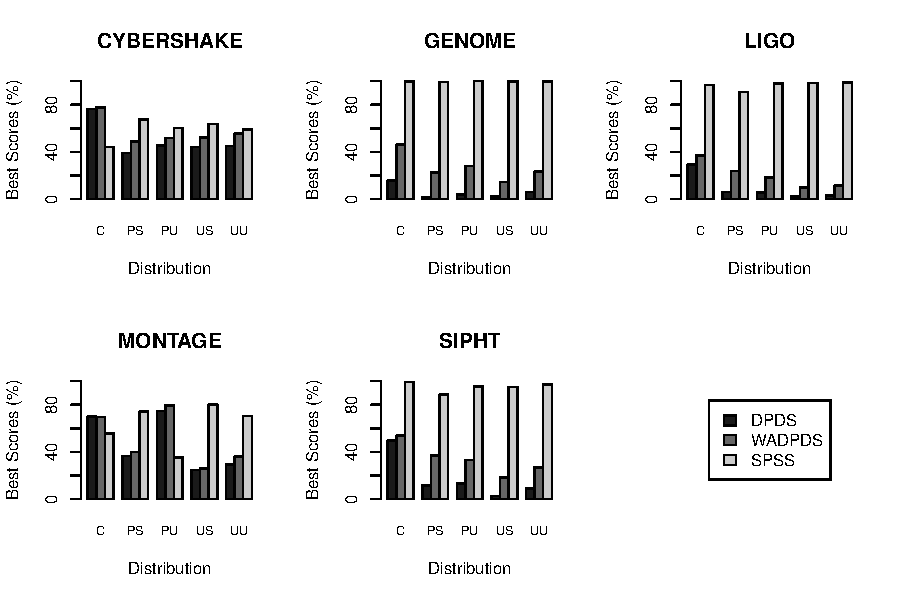
\includegraphics[width=\textwidth]{run-finish-variations-test-0-output-distributions}
    \caption{Percentage of high scores achieved by each algorithm on different ensemble types for all five applications. C = Constant ensembles, PS = Pareto Sorted ensembles, PU = Pareto Unsorted ensembles, US = Uniform Sorted ensembles, and UU = Uniform Unsorted ensembles.} 
    \label{fig:distributions}
\end{figure*}

There are several interesting things to notice about
Figure~\ref{fig:distributions}. The first is that, in most cases, SPSS
significantly outperforms both dynamic algorithms (DPDS and WA-DPDS). This is
attributed to the fact that SPSS is able to make more intelligent scheduling
and provisioning decisions because it has the opportunity to compare different
options and choose the one that results in the best outcome. In comparison,
the dynamic algorithms are online algorithms and are not able to project into
the future to weigh the outcomes of their choices.

The second thing to notice about the figure is that, for constant ensembles,
the dynamic algorithms perform significantly better relative to SPSS than for
other ensemble types. This is a result of the fact that, since all of the
workflows are of approximately the same size and shape, the choice of which
workflow to execute next has little impact on the final result.

Another thing to notice about this experiment is that the workflow-aware
algorithms (WA-DPDS and SPSS) both perform better in most cases than the
simple online algorithm that uses resource utilization alone to make
provisioning decisions (DPDS). This suggests that there is a significant value
in having information about the structure and estimated runtime of a workflow
when making scheduling and provisioning decisions.

Finally, it is interesting to see that, for Montage and CyberShake, the
relative performance of SPSS is significantly less than it is for other
applications. We attribute this to the structure of Montage and CyberShake.
The workflows for both applications are very wide relative to their height,
and both have very short-running tasks. As a result of these two
characteristics, the Montage and CyberShake applications have very short
critical paths and look more like bag-of-tasks applications, which are easier
to execute than more structured applications. DPDS and WA-DPDS are able to
pack more of the tasks into the available budget and deadline because there
are a) more choices for where to place the tasks, and b) the different choices
have a smaller impact on the algorithms' ability to execute the workflow
within the constraints. In addition, the short critical paths put SPSS at a
disadvantage. Because of the way SPSS assigns deadlines to individual tasks,
it is prevented from starting workflows late, which prevents it from packing
tasks into the idle VM slots at the end of the schedule.


\subsection{Task Granularity}
\TODO{Should we remove this section?}

In the last experiment we noted that, for Montage and CyberShake, the short
runtimes of their tasks made the dynamic algorithms perform better relative to
SPSS. In order to test this theory we adjusted the granularity of the tasks in
several Montage and CyberShake ensembles to see how this would affect the
relative performance of the algorithms. The granularity adjustment was
achieved by multiplying the runtime of each task by a fixed scaling factor.

Figure~\ref{fig:stretching} shows the relative performance of the algorithms
as the scaling factor is increased from 1 to 16. The figure only shows results
for the CyberShake application with pareto unsorted ensembles, but similar
results were found for other ensemble types for both Montage and CyberShake.
Each data point in the figure represents 500 simulations (5 ensembles with 10
budgets and 10 deadlines). The best scores percent was calculated the same way
as it was for Figure~\ref{fig:distributions}.

The figure shows that, as the scaling factor increases beyond 2, the relative
performance of SPSS surpasses that of the dynamic algorithms. Similar results
were found for other ensemble types for both applications. This result
suggests that, in general, for fine-grained workflows the dynamic algorithms
will produce better scores, and for coarse-grained workflows SPSS will produce
better scores.

\begin{figure}[tb]
    \centering
    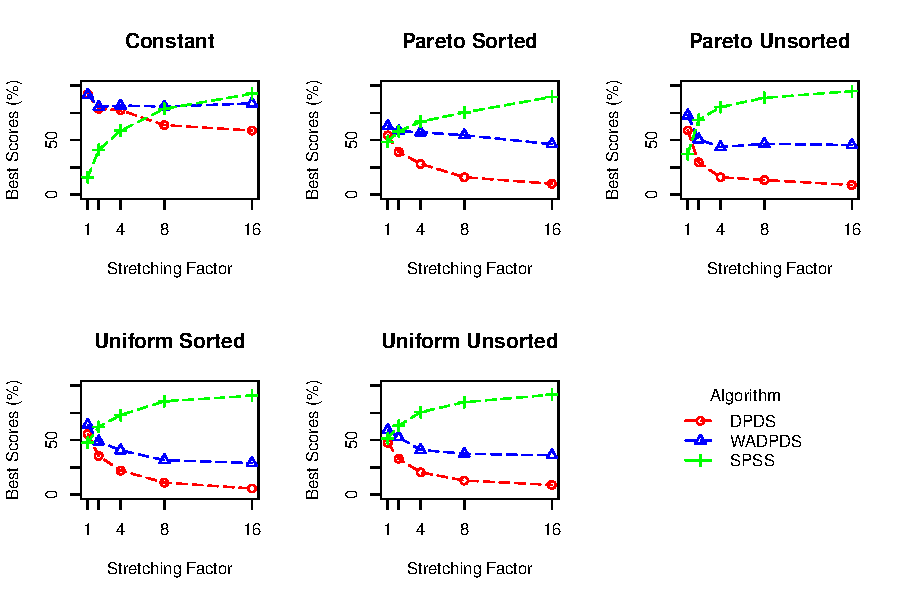
\includegraphics[width=0.3\textwidth]{stretching_cybershake}
    \caption{Percentage of high scores achieved by each algorithm for pareto 
    unsorted CyberShake ensembles when task runtime is scaled by a constant 
    factor. A scaling factor of $x$ means that the runtime of tasks in each 
    workflow was multiplied by $x$.}
    \label{fig:stretching}
\end{figure}


\subsection{Inaccurate Task Runtime Estimates}
\label{sec:variances}

Both of the workflow-aware algorithms rely on estimates of task runtimes to
make better scheduling and provisioning decisions. In practice, however, these
estimates are often inaccurate. Given inaccuate estimates, the question is:
How do errors in task runtime estimates impact the performance of our
scheduling and provisioning algorithms? We created an experiment to measure
how introducing uniform errors in these estimates affects the ability of the
algorithms to achieve the desired budget and deadline constraints. 

\TODO{Update the description of the experiment in this paragraph if necessary}

This experiment used a single application, Montage, and a single ensemble
type, uniform unsorted. This application and ensemble type was chosen
arbitrarily for simplicity. It is expected that the application and ensemble
type have little impact on how well the algorithms are able to stay within
constraints.

The actual runtime of each task is adjusted in the simulation by adding a
random error to the estimated runtime of $\pm p\%$. Since the sampling is done
uniformly, we expect to get just as many overestimates as underestimates in
any given simulation.

Figure~\ref{fig:variances} shows the results of simulations for estimate
errors ranging from $0\%$ to $50\%$. These simulations were done for 10
ensembles of 50 workflows using 10 budgets and 10 deadlines for each error
value and algorithm (3000 simulations per error value). The figure shows box
plots of the ratio of actual cost to budget and actual makespan to deadline.
The actual cost and makespan are the simulated cost and makespan of the
ensemble. The ratio of actual values to constraints indicates whether the
actual value exeeded the constraint: Values less than 1 indicate that the
constraint was not exceeded, and values greater than 1 indicate that the
constraint was exceeded.

Figure~\ref{fig:variances}.a shows the ratio of actual cost to budget. This
figure illustrates two important algorithm characteristics. First, the dynamic
algorithms very rarely exceeded the budget, even with very large errors. This
indicates that the dynamic algorithms are able to adapt to uncertainties at
runtime to ensure that the constraints are not exceeded, even when the quality
of information available to them is low. Second, unlike the dynamic
algorithms, the static algorithm frequently exceeded the budget constraint; by
large amounts in some cases. This is a result of the fact that the static
algorithm makes all of its decisions before execution and is not able to adapt
to changing circumstances.

%The SPSS plan describes what tasks to execute on which VMs, but not when to
%execute them. At runtime, the worklow engine is forced to spend extra money
%to extend the runtime of some VMs so that all of the tasks assigned to that
%VM can be completed. At the same time, other VMs can be terminated early
%because the tasks they were assigned finished earlier than expected. However,
%because of dependencies in the workflow, the latter case is less likely to
%happen, which causes gaps in the schedule. So the net result is that the
%overall cost is increased.

Figure~\ref{fig:variances}.b shows the ratio of actual makespan to budget. The
interesting thing to notice about this figure is that, for all three
algorithms, the deadline constraint is rarely exceeded, even in cases with
very poor quality estimates. For the dynamic algorithms this is a result of
the fact that they can adapt to poor estimates. For the static algorithm this
is a result of the way that SPSS schedules workflows, and not of a
particularly clever optimization. The SPSS algorithm tends to schedule
workflows early, using up the budget long before the deadline is reached. This
is a consequence of the deadline distribution function in SPSS, which prevents
workflows from starting late. This is shown by the gantt chart in
Figure~\ref{fig:algorithm-example}.b, which illustrates how SPSS tends to pile
up workflows at the beginning of the timeline. In comparison, the dynamic
algorithms tend to spread out workflow starts over the entire duration as
shown in Figure~\ref{fig:algorithm-example}.a. The consequence of this
behavior is that SPSS plans tend to use up the budget but leave plenty of time
before the deadline. So when the runtime of the plan is increased by
introducing errors, the SPSS plan has some room to expand without exceeding
the deadline.

Note that the algorithms have \textit{not} been changed to account for
inaccurate runtime estimates in this experiment. It is likely that better
performance could be achieved if the algorithms were given a hint as to the
accuracy of the task runtimes. Investigating that optimization is left for
future work. The goal here is to determine how well the current algorithms are
able to stay within the constraints given inaccurate task runtime estimates.

%It is possible that the static algorithm could be modified to add more
%breathing room in the schedule to account for situations where the runtime
%estimates may be inaccurate. Such a modification would result in slightly
%worse scores when the estimates are good, but would improve scores when the
%estimates are bad. Alternatively, the SPSS algorithm could be modified to
%generate a plan that specifies when to provision and deprovision each VM. In
%that case the workflow engine could be prevented from exceeding the budget
%and deadline constraints, but would prevent some workflows from finishing,
%which may significantly decrease the score. These two modifications are
%subjects for future work.

\begin{figure*}[tb]
    \centering
    \subfloat[Ratio of Actual Cost to Budget]{
        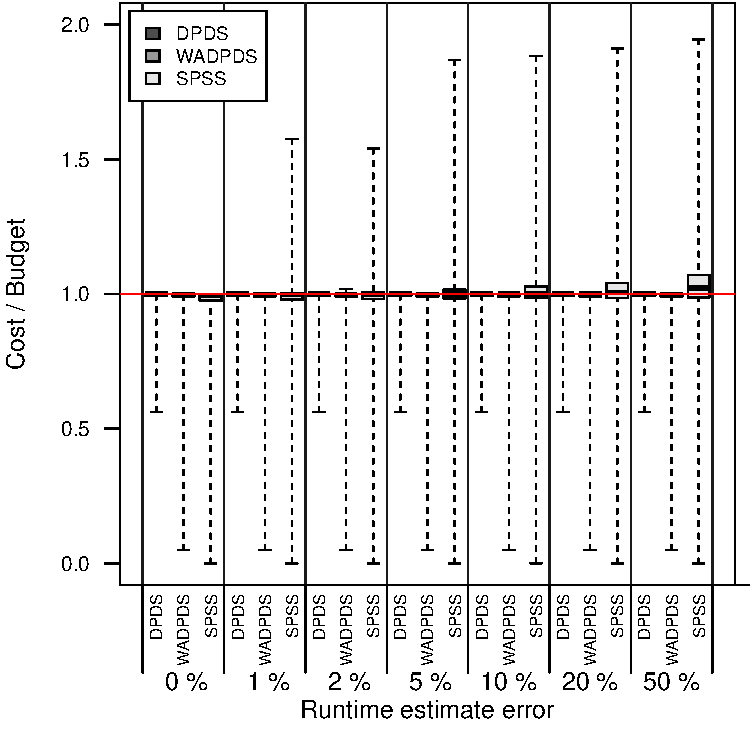
\includegraphics[width=0.4\textwidth]{run-finish-variations-test-0-output-cost-all}
    }
    \hspace{2cm}
    \subfloat[Ratio of Actual Makespan to Deadline]{
        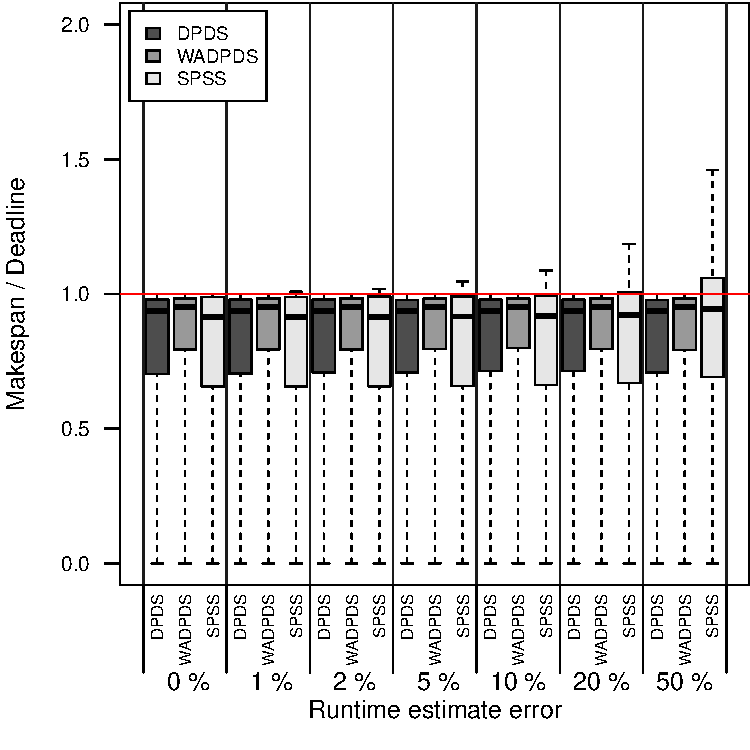
\includegraphics[width=0.4\textwidth]{run-finish-variations-test-0-output-makespan-all}
    }
    \caption{Boxplots for budget and deadline ratios when runtime estimate 
    error varies from $\pm$0\% to $\pm$50\% for all three algorithms. Values 
    greater than 1 indicate that the budget/deadline constraint was exceeded.}
    \label{fig:variances}
\end{figure*}


\subsection{Provisioning Delays}
\label{sec:delays}

One important issue to consider when provisioning resources in the cloud is
the amount of time between when a resource is requested, and when it actually
becomes available to the application. Typically these provisioning delays are
on the order of a few minutes, and are highly dependent upon the architecture
of the cloud system and/or the size of the user's VM image~\cite{Nurmi2008b}.

We assume that resources are billed from the minute that they are requested
until they are terminated, and not from the moment that they become available.
As a result, provisioning delays have an impact on both the cost (budget
constraint) and makespan (deadline constraint) of the ensemble.

\TODO{Update the following paragraph depending on what results Maciek included}

Figure~\ref{fig:delays} shows the ratios of actual values to constraints when
the provisioning delay is increased from 0 seconds up to 15 minutes. These
simulations were done using 10 uniform unsorted ensembles of 50 workflows from
the Montage application, using 10 deadlines (1000 simulations per algorithm
and provisioning delay). As in Figure~\ref{fig:variances}, the y-axis in each
plot represents the ratio of the actual simulated value to the constraint
value for the budget constraint (actual cost) or the deadline constraint
(actual makespan). These ratios indicate how frequently and by how much the
actual simulated values exceeded (or did not exceed) the constraints.

\begin{figure*}[tb]
    \centering
    \subfloat[Ratio of Actual Cost to Budget]{
        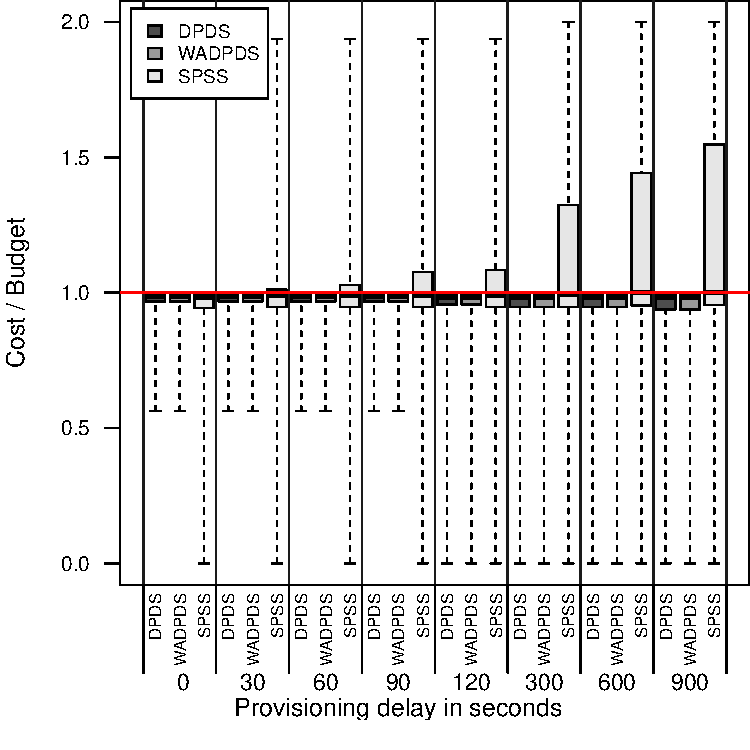
\includegraphics[width=0.4\textwidth]{run-finish-delays-test-0-output-cost-montage}
    }
    \hspace{2cm}
    \subfloat[Ratio of Actual Makespan to Deadline]{    
        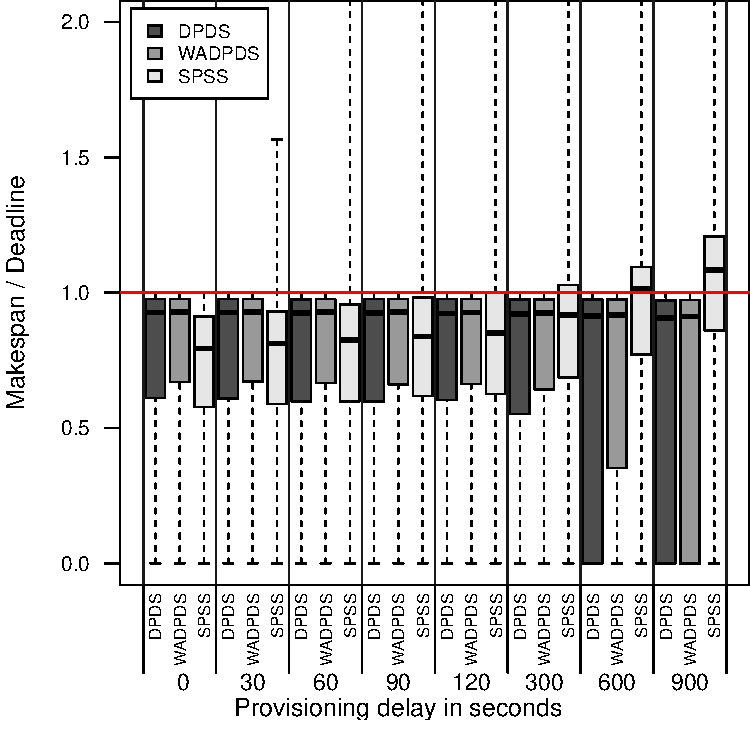
\includegraphics[width=0.4\textwidth]{run-finish-delays-test-0-output-dagfinish-montage}
    }
    \caption{Boxplots for budget and deadline ratios when provisioning delay 
    varies from 0 seconds to 15 minutes for all three algorithms. Values 
    greater than 1 indicate that the budget/deadline constraint was exceeded.}
    \label{fig:delays}
\end{figure*}

\TODO{Update this next paragraph depending on what Maciek included in the figure. The results seem to have changed.}

The effect of provisioning delays on workflow performance is similar to that of inaccurate runtime estimates: when the delays are small, all algorithms are able to produce results within the constraints, but when the delays are larger, the dynamic algorithms are able to adapt to avoid exceeding the constraints while the static algorithm is not. The explanation for this behavior is also similar. The difference is that, a very small error in runtime estimates has little impact on the budget, while a very small provisioning delay has a large impact on the budget. Figure~\ref{fig:delays}.a shows that even for a very short provisioning delay of 30 seconds (usually it takes more than than 30 seconds just to boot a VM), the SPSS algorithm exceeds the budget by as much as a factor of 2, and has a distribution with an upper quartile of 1.5 times the budget. In the case of delays more than 5 minutes, which is more typical of what has been observed on academic infrastructure clouds~\cite{Juve2011} such as Magellan~\cite{Magellan} and FutureGrid~\cite{FutureGrid}, fully three quarters of the simulations exceeded the budget. With the exception of a few outliers for 10 and 15 minute delays, the dynamic algorithms consistently met the budget and deadline constraints.

% Figure~\ref{fig:delays_scores} shows the relative performance as a
% percentage of the number of high scores achieved by each algorithm as the
% provisioning delay increases. This figure shows that, as the delay
% increases, the relative performance of the static algorithm increases as
% well. This behavior is a result of the fact that the static algorithm is, in
% essence, cheating by using more time and money than the dynamic algorithms.
% In the previous section we showed how the relative performance of the
% algorithms remains the same when a uniform error is applied to the runtime
% constraints. In that case, the dynamic algorithms adapted to the error by
% rearranging the schedule to accomplish the same amount of work given the
% same deadline and budget. In this case, the dynamic algorithms adapt by
% performing less work (executing fewer workflows) to remain within the
% constraints while accounting for the delays. In both cases, the static
% algorithm completed the same amount of work, but did so by exceeding the
% constraints.

% \begin{figure}[ht]
%   \centering
%   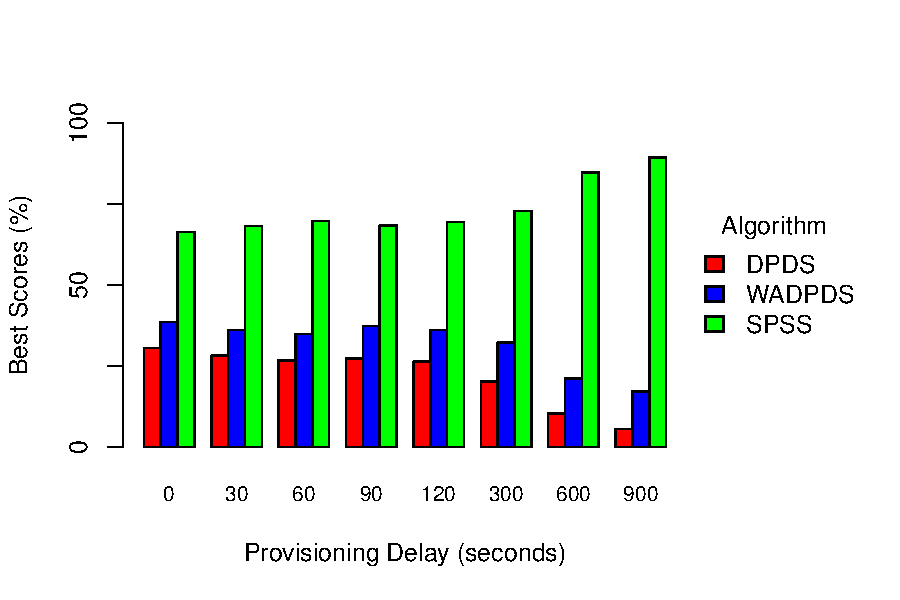
\includegraphics[width=0.5\textwidth]{delays_scores}
%   \caption{Percentage of high scores achieved by each algorithm on Montage 
%   with uniform unsorted ensembles when provisioning delay varies from 0 
%   seconds to 15 minutes.}
%   \label{fig:delays_scores}
% \end{figure}

\TODO{Update this paragraph when Maciek explains what was included in the plot.}

This behavior suggests that SPSS is far too sensitive to provisioning delays in its current form to be of practical use in real systems. It is likely, as was the case for inaccurate runtime estimates, that modifying the SPSS algorithm would improve its performance for provisioning delays. In fact, since provisioning operations are infrequent (because all the algorithms tend to provision resources for a long time), it is likely that the performance of SPSS could be improved significantly by simply adding an estimate of the provisioning delay to its scheduling function. Such an estimate may not have to be particularly accurate to get good results, and developing an estimate from historical data should be relatively simple. Testing this idea is left for future work.


\subsection{Task Failures}
\label{sec:failures}

Running workflows consisting of large numbers of tasks on distributed systems
often results in failures. The goal of the next experiment was
to assess the behavior of the algorithms in the presence of task execution
failures by introducing a failure model into the simulator. The model is
characterized by a failure rate $f$ that defines the probability that a task
will fail. The failure time of the task is determined by randomly sampling a
value between the task start time and finish time. If the task fails, it is reported to
the workflow engine, which retries the task until it succeeds. The dynamic algorithms
re-add the task to the priority queue (queue $P$ in Algorithm~\ref{alg:ds})
so that it can be resubmitted by the scheduler. The SPSS algorithm immediately 
resubmits the failed task to the same VM that was selected in the plan.

\begin{figure*}[tb]
    \subfloat[Ratio of Actual Cost to Budget]{
        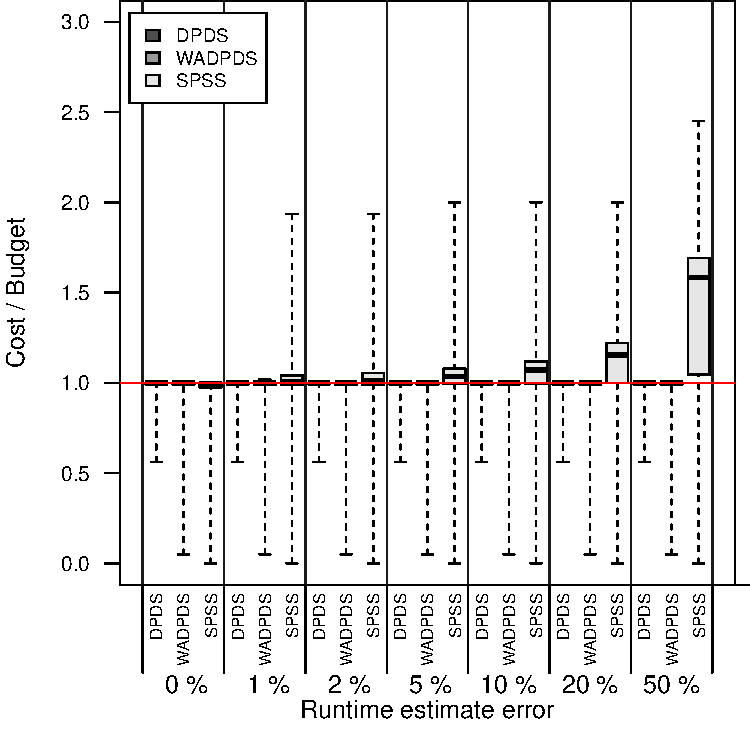
\includegraphics[width=0.4\textwidth]{run-finish-failures-test-0-output-cost-all}
    }
    \hspace{2cm}
    \subfloat[Ratio of Actual Makespan to Deadline]{
        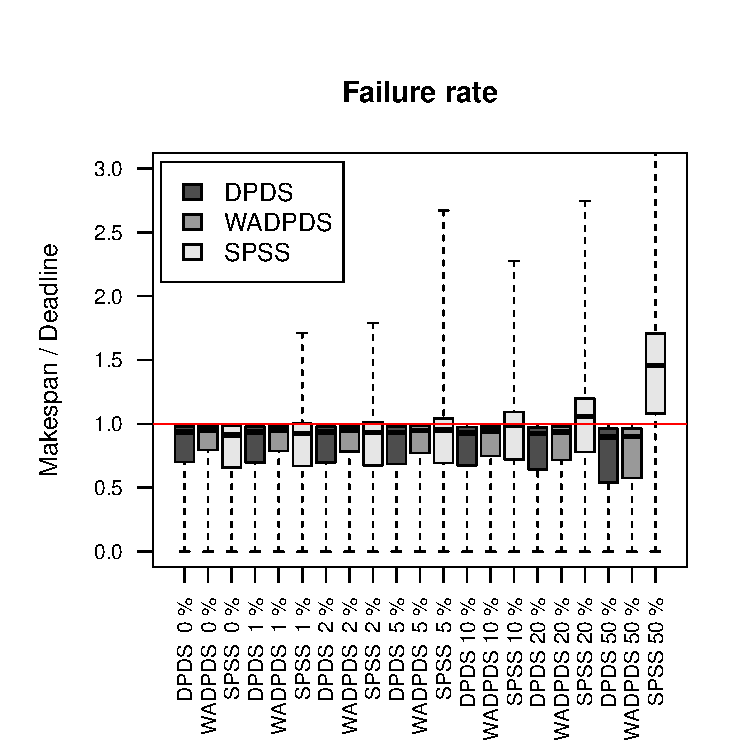
\includegraphics[width=0.4\textwidth]{run-finish-failures-test-0-output-makespan-all}
    }
    \caption{Boxplots for budget and deadline ratios when failure rate varies
    from 0\% to 50\% for all three algorithms. Values greater than 1 indicate 
    that the budget/deadline constraint was exceeded.}
    \label{fig:failures}
\end{figure*}

\TODO{Include a description of the ensembles that were simulated.}

Fig.~\ref{fig:failures} shows the ratios of actual values to constraints when
the failures are introduced. The high failure rates have a high impact on the
performance of the static algorithm and can degrade the solution considerably.
Comparing Fig.~\ref{fig:failures} to Figs.~\ref{fig:variances}
and~\ref{fig:delays} one may conclude that failures are worse than
provisioning delays and runtime estimate errors, since their impact is larger.
However, small failure rates (below 10\%) do not cause constraint overruns
larger than 10\%. We consider higher failure rates as rare events that suggest
a significant system malfunction or invalid selection of resources.


\subsection{SPSS Planning Time}

Unlike the dynamic algorithms, which execute their scheduling and provisioning logic at runtime, the SPSS algorithm plans out its provisioning and scheduling decisions ahead of workflow execution. Because SPSS involves more complicated logic than the dynamic algorithms, it is important to understand what impact this has on execution time.

Figure~\ref{fig:spss_planning_time} shows the SPSS planning time for ensembles of 100 workflows with five different workflow sizes: 50, 200, 400, 600, and 800 tasks. The ensembles were generated using a constant distribution equal to the workflow size desired. Two different applications were used: SIPHT and CyberShake. Each box summarizes the results of 2 applications, 10 random seeds, 10 budgets and 10 deadlines, or 2000 simulations per box.

Figure~\ref{fig:spss_planning_time} shows that, for small workflows, the SPSS planning time is reasonable, taking on the order of tens of seconds to a few minutes. For larger ensembles of large workflows, however, the SPSS planning time can easily reach 10 minutes. Considering that the largest workflows used in this experiment are still relatively small (maximum of 800 tasks), and that real workflows are often much larger (workflows with tens of thousands of tasks are common, and workflows with hundreds of thousands or millions of tasks are not impossible), it is unlikely that SPSS will be practical for ensembles of very large workflows.

\begin{figure}[tb]
    \centering
    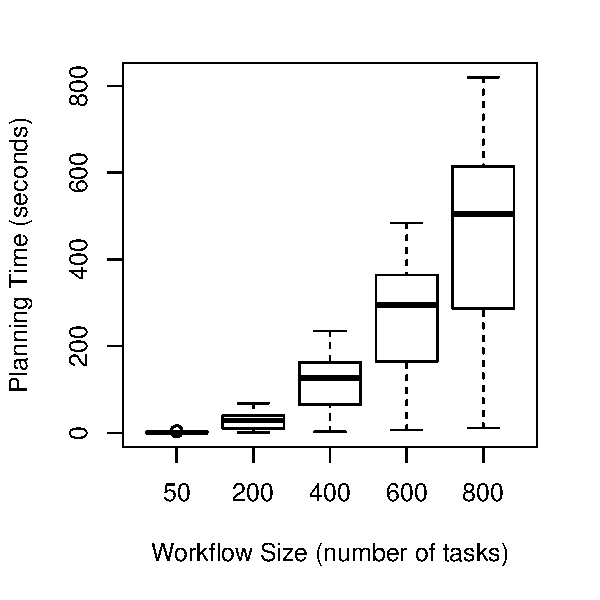
\includegraphics[width=0.3\textwidth]{spss_planning_time}
    \caption{Planning time of SPSS algorithm for ensembles of 100 workflows and different workflow sizes.}
    \label{fig:spss_planning_time}
\end{figure}

The algorithmic complexity of SPSS is $O(n^2)$, where $n$ is the number of tasks in the ensemble. This derives from the fact that, for each task, SPSS considers scheduling the task on the cheapest available slot, which involves scanning all of the available slots on all the VMs. Since the number of available slots, in the worst case, is proportional to the number of tasks scheduled (because scheduling a task splits an existing slot into at most two slots), the complexity of SPSS is $O(n^2)$. In comparison, the dynamic algorithms all have a more scalable complexity of $O(n)$. DPDS only examines the tasks in the workflow once when they are scheduled, and WA-DPDS examines them twice: once in the admissions algorithm, and once when they are scheduled. This makes the dynamic algorithms a better fit for larger workflows and ensembles even though they may not produce results that are as good as SPSS.

It may be possible to optimize SPSS to reduce its runtime by, for example, clustering the workflow to increase task granularity, which would decrease the ratio of planning time to ensemble makespan. It may also be possible to reduce the complexity of SPSS by employing more sophisticated data structures to store the available slots. Investigating these topics is left for future work.


\section{Conclusions and Future Work}
\label{sec:conclusions}

In this paper we addressed the interesting and important new problem of scheduling and resource provisioning for scientific workflow ensembles on IaaS clouds. The goal of this work is to maximize the number of prioritized workflows that can be completed given budget and deadline constraints.

%This problem differs from previous work on grid and utility grid scheduling in that cloud infrastructures provide more control over provisioning, so that the number of resources can be adjusted according to the requirements of the application. Therefore the problem space becomes larger; it requires not only an efficient mapping of tasks to available resources, but also the selection of the best resource provisioning plan.

%Formulating the problem as a maximization of the number of prioritized workflows completed from the ensemble is also novel and requires workflows to be admitted or rejected based on their estimated resource demands. We believe that this bi-constrained problem is highly relevant because such constraints are commonly imposed on many real-world projects. The approach is also directly applicable to grid environments that provide resource reservations and charge service units for resource use.

We developed three algorithms to solve this problem: two dynamic algorithms, DPDS and WA-DPDS, and one static algorithm, SPSS. The algorithms were evaluated via simulation on ensembles of synthetic workflows, which were generated based on statistics from real scientific applications.

The results of our simulation studies indicate that the two algorithms that take into account the structure of the workflow and task runtime estimates (WA-DPDS and SPSS) yield better results than the simple priority-based scheduling strategy (DPDS), which makes provisioning decisions based purely on resource utilization.

In cases where there are no provisioning delays, task runtime estimates are good, and failures are rare, we found that the static algorithm, SPSS, performs significantly better than both dynamic algorithms. However, when conditions are less than perfect, the static plans produced by SPSS are disrupted and it frequently exceeds the budget and deadline constraints. In comparison, the dynamic algorithms are able to adapt to a wide variety of conditions, and rarely exceed the constraints even with long delays, poor estimates, and high failure rates.

%In addition, we found that SPSS tends to perform better on coarse-grained workflows than the dynamic algorithms. For wide, fine-grained workflows, such as CyberShake and Montage, however, the dynamic algorithms frequently produce performance that is as good or better than SPSS, because they are better able to pack the smaller tasks onto idle VMs close to the deadline than SPSS, which distributes deadlines to tasks in a way that prevents them from starting late.

%For very large workflows and ensembles, we found that the planning time of the SPSS algorithm is prohibitive. SPSS often took 10 minutes or more to plan ensembles of 100 workflows with 800 tasks each. This suggests that ensembles of workflows with tens of thousands of tasks, which are commonly encountered in real workflow applications, would take many hours to plan using SPSS. This makes the dynamic algorithms much more attractive for large scale problems.

This study suggests several areas for future work. Our current approach models data access as part of the task execution time and does not consider data storage and transfer costs. In the future we plan to extend the application and infrastructure model to  include the various data storage options available on clouds. A previous experimental study \cite{Juve2010} suggests that the data demands of scientific workflows have a large impact on not only the execution time, but also on the cost of workflows in commercial clouds. We also plan to investigate heterogeneous environments that include multiple VM types and cloud providers, including private and community clouds, which will make the problem even more complex and challenging.

%The results of this study can be applied to develop tools that assist researchers in planning their large-scale computational experiments. The estimates of cost, runtime, and number of workflows completed that can be obtained from both the static algorithms and from the simulation runs, constitute valuable hints for planning ensembles and evaluating the associated trade-offs.


%\section*{Acknowledgments}
%Acknowledgements go here.


% ACM style
%\bibliographystyle{abbrv}

% IEEE style
\bibliographystyle{IEEEtran}

% This balances the columns by inserting a column break at the given reference
\IEEEtriggeratref{19}

\bibliography{paper}

%\appendix
%\section{Headings in Appendices}

%\balancecolumns

\end{document}
